
V oblasti teórie strojového učenia sa zaoberáme učením; formalizujeme ho,
navrhujeme rôzne algoritmy schopné tohto učenia, analyzujeme ako rýchlo
sa tieto algoritmy učia, ... Čo to ale vlastne je to ``učenie'', a ako sa
nad týmto konceptom dá zamýšľať?

Začnime tým, že si vybavíme, čo všetko sa nám spája s učením. Napríklad
učenie sa na skúšky, ktoré pre niektorých vyzerá tak, že sa snažia si
zapamätať všetkých $80$ strán skrípt naspamäť. Alebo keď sa snažíme
naučiť novú skladbu na klavíri: hráme ju znova a znova, až kým v tom
nie sme dobrí. Alebo trénovanie na dôležitý zápas vo futbale, ...

Vidíme teda, že učenie je zložitý koncept. Konkrétne detaily toho, ako
presne sa učíme (resp. prečo to funguje), sú známe málo ľuďom. Avšak
vidíme, že jednotlivé ``učenia'' mali niečo spoločné: nejaká aktivita
sa opakovala veľakrát, a čím viackrát sa zopakovala, tým lepší bol
výkon. Zároveň ale nechceme, aby sa zakaždým odohralo to isté; nová
skúsenosť je dôležitou súčasťou učenia.

Ak by sme len tak vychrlili nejakú definíciu, ktorá nám príde rozumná,
riskujeme, že nebude ``sedieť s našou intuíciou'', alebo nebude dostatočne
všeobecná. Kvôli tejto zložitosti teda namiesto toho, aby sme zachytili
``učenie'' v jednej definícii, študujeme veľa rôznych modelov učenia,
ktoré sú aplikovateľné v rôznych kontextoch. Pod ``modelom'' rozumieme
akúsi hračku, zjednodušený mentálny obraz, s ktorým sa jednoducho pracuje
a zároveň ``sedí s našou intuíciou''. Takto síce nijak neručíme, že pokrývame
``všetko učenie''; čím viac viet a teorém v rôznych modeloch ale dokážeme,
tým lepší budeme mať obraz o tom, čo to učenie je.

My sa v týchto skriptách budeme zaoberať hlavne oblasťou \emph{učenia s
učiteľom}. Uvedieme hlavný model (tzv. \emph{statistical learning framework}),
s ktorým budeme pracovať, a v prípade potreby rozširovať/dolaďovať.

Predstavme si, že chceme vedieť na základe nejakých vstupných dát (ktoré
budeme spravidla označovať $x$) predpovedať výstupné dáta (označované $y$).
Napríklad chceme na základe rozlohy bytu vedieť predpovedať jeho cenu.
Alebo vedieť z obrázku (vo formáte $32 \times 32$ čiernobielych pixelov)
povedať, či sa v ňom nachádza mačka alebo nie.

Snažíme sa teda zachytiť nejaký vzťah medzi dátami $x$ a $y$. To, akým
spôsobom to budeme robiť, je nasledovné: nejakým procesom $P$ získame $t$
\emph{trénovacích príkladov} $(x_1, y_1), \ldots, (x_t, y_t)$. Na základe
týchto príkladov budeme chcieť navrhnút nejakú funkciu $h$, ktorá bude
vedieť podľa vstupu $x$ predpovedať výstup $y$ s dostatočnou presnosťou.

Prirodzený spôsob, akým môžeme merať úspešnosť funkcie $h$, je podľa
toho, ako sa jej darí na našich $t$ príkladoch. Prístupu, kde hľadáme
funkciu, ktorej sa čo najlepšie darí na trénovacích príkladoch, hovoríme
\emph{empirical risk minimization} (skrátene ERM). Dobrá funkcia $h$ ale
bude schopná aj \emph{generalizovať}: bude sa jej dariť na ďalších
dátach, ktoré vieme získať tým istým procesom $P$.

Schopnosť generalizácie je jednou z najdôležitejších vlastností, ktoré
od trénovania pomocou techník strojového učenia požadujeme. Predstavme si,
že by sme funkciu $h$ zostrojili tak, že si ``zapamätáme'' všetky trénovacie
príklady: ak je na vstupe $x$, ktoré bolo medzi trénovacími príkladmi,
vrátime príslušné $y$. Takáto funkcia $h$ má zrejme nulovú chybu na
trénovacích príkladoch (pokiaľ pre jedno $x$ existuje vždy len
jedno správne $y$), ale mimo nich sa jej vôbec nebude dariť.

Vidíme teda, že ERM vo svojej holej podstate nefunguje. Problém je v tom,
že neobmedzujeme to, aké funkcie považujeme sa ``kandidátov'': nič
nezaručuje, že informácia z trénovacích príkladov sa prenesie aj na
ostatné príklady. Obmedzíme teda množinu funkcii, ktoré uvažujeme,
na nejakú užšiu skupinu, ktorú nazveme \emph{množina hypotéz}.

Napríklad si predstavme, že hľadáme funkciu $f : \R \to \R$ a dostali
sme trénovacie príklady $(0, 0)$ a $(1, 1)$. Ak o probléme nič ďalšie
nevieme, tak nevieme povedať nič o tom, ako sa bude $f$ správať pre
$x \not\in \{0, 1\}$. Ak ale vieme, že hľadáme neklesajúcu funkciu
s oborom hodnôt $\{0, 1\}$, tak vieme, že $f(x) = 0$ pre $x \leq 0$,
$f(x) = 1$ pre $x \geq 1$, a niekde v intervale $(0, 1)$ sa to ``láme''.

Tým, že sme obmedzili množinu hypotéz, sme v podstate zaviedli
\emph{inductive bias}: predpoklady, ktoré využívame na to, aby
sme odvodili výsledky aj na tých vstupoch, ktoré sme ešte nevideli.


\section{Štatistický model učenia, základné definície a predpoklady}
\label{ch1:stat_lr_fw}

Množinu všetkých možných vstupov označíme $X$, niekedy jej budeme hovoriť aj
\emph{množina inštancií}. Množinu všetkých možných výstupov označíme $Y$.
Proces, ktorým získavame dáta $(x, y)$, vieme formalizovať pomocou
pravdepodobnostného rozdelenie $P$ nad priestorom $X \times Y$, ktoré
každému možnému pozorovaniu priradí nejakú pravdepodobnosť (resp. hustotu
pravdepodobnosti v prípade spojitého rozdelenia).

Trénovacie príklady získame ako $t$ nezávislých vzoriek z rozdelenia $P$.
Množinu trénovacích príkladov budeme volať \emph{trénovacia
množina} a označíme ju $T$. (Z matematického hľadiska to ale nie je
množina, kedže jedna dvojica $(x, y)$ sa medzi
trénovacími príkladmi môže vyskytovať viackrát. Pre jednoduchosť to
ale budeme nazývať množinou.) 

\begin{remark}[Skrátené zápisy stredných hodnôt.]
Vzhľadom k tomu, že pravdepodobnostné rozdelenie $P$ nám bude slúžiť v tomto
texte ako ``univerzálny'' model sveta, zápisy stredných hodnôt budeme
zjednodušovať nasledovne:

\begin{itemize}
  \item ak sa stredná hodnota berie cez príklady z rozdelenia $P$:
    $$ \E_{(x, y) \sim P} \equiv \E_{x, y} $$
%  \item ak sa stredná hodnota berie cez všetky trénovacie príklady
%    z množiny $T$:
%    $$ \E_{(x, y) \in T} \equiv \E_{x_i, y_i} $$
  \item ak sa stredná hodnota berie cez všetky možné trénovacie
    množiny veľkosti $t$:
    $$ \E_{T \in P^t} \equiv \E_T $$
\end{itemize}
Podobné skrátené zápisy budeme používať aj pri pravdepodobnostiach
a pod.
\end{remark}

Postup, ktorým zostrojíme funkciu $h$, vieme formalizovať ako algoritmus $L$,
ktorý na vstupe dostane niekoľko trénovacích príkladov
$(x_1, y_1), \ldots, (x_t, y_t)$, a na výstupe vráti funkciu $h : X \to Y$,
ktorú budeme volať \emph{hypotéza}. Táto hypotéza bude pochádzať z
takzvanej \emph{množiny hypotéz}, ktorú označíme $H$.

\subsection{Chyba hypotézy, očakávaná trénovacia a testovacia chyba}

Chybu hypotézy budeme vyhodnocovať
pomocou \emph{chybovej funkcie} $\err : Y \times Y \to \R^+_0$,
pričom $\err(y, y')$ vyjadruje, ako veľmi
sa od seba líšia výstupy $y$ a $y'$.

Pri klasifikácii sa naša hypotéza vždy buď trafí, alebo netrafí do
správnej odpovede.  Správnej
odpovedi priradíme chybu $0$, nesprávnej odpovedi chybu $1$:
$$
  \err(y, y') = \left\{
    \begin{array}{ll}
      0, & \text{ak}\ y = y' \\
      1, & \text{inak}
    \end{array}
  \right.
  .
$$

%Potom sa nám viacero vzorcov pre chyby zjednoduší: testovacia chyba
%hypotézy je
%$$\Err(h) = \E_{(x, y) \sim P} \left[ \err(h(x), y) \right] = \prob_{(x, y) \sim P} \left( h(x) \neq y \right),$$
%a podobne sa dá zjednodušiť aj trénovacia chyba.

Pri regresii budeme v nasledujúcom texte používať funkciu
$\err(y,y')=(y-y')^2$ (takzvaná $L_2$ chybová funkcia), často sa používa
aj funkcia $\err(y,y')=|y-y'|$ (takzvaná $L_1$ chybová funkcia).

\emph{Chyba na jednom príklade.} Keď dostaneme nejaký príklad $(x, y)$,
vieme zmerať, ako veľmi sa naša hypotéza $h$ na tomto vstupe pomýlila,
ako $\err(h(x), y)$. \emph{Trénovacia chyba} je chyba,
ktorú hypotéza nadobúda na trénovacej množine. Budeme ju
označovať $\Err$, a vypočítame ju nasledovne:
$$\Err_T(h) = \frac{1}{t} \cdot \sum_{i=1}^t \err(h(x_i), y_i).$$
%Tento zápis sa dá chápať aj tak, že trénovaciu množinu interpretujeme
%ako pravdepodobnostné rozdelenie, pričom pravdepodobnosť každého príkladu
%je úmerná tomu, koľkokrát sa v množine vyskytuje. Niekedy túto chybu
%budeme zapisovať aj $\Err_T(h)$.

\emph{Očakávaná testovacia chyba hypotézy} je očakávaná chyba
na náhodne vybranom príklade z rozdelenia $P$.
Túto chybu budeme tiež označovať $\Err$,
a vypočítame ju nasledovne:
$$\Err_P(h) = \E_{(x, y)\sim P} \left[ \err(h(x), y) \right].$$
Rozdelenie $P$ bude obvykle jasné z kontextu, v takom prípade
budeme skrátene písať $\Err(h)$.

\subsection{Predpoklady o trénovacom algoritme}
\label{ch1:asses}

Doteraz sme neriešili, ako má vyzerať trénovací algoritmus $L$. Vo
všeobecnosti, takýto algoritmus dostane na vstupe trénovaciu množinu
$T$ pozostávajúcu z $t$ trénovacích príkladov a množinu hypotéz $H$,
ktorá charakterizuje všetky možné ``použiteľné'' hypotézy. Výstupom
takéhoto algoritmu má byť jedna funkcia $h\in H$, ktorú nazveme
natrénovaná hypotéza.

Vo všeobecnosti, uvažovať vlastnosti ľubovoľného takého algoritmu $L$
je veľmi ťažké. Intuitívne je jasné, že hypotéza, ktorú dá algoritmus
na výstupe, by mala určite mať malú trénovaciu chybu pre trénovaciu
množinu $T$. Kým pre niektoré množiny hypotéz $H$ môže byť nájdenie
takej hypotézy pomerne priamočiare (ako napríklad nájdenie funkcie
minimalizujúcej $L_2$ trénovaciu chybu na množine všetkých lineárnych
funkcií), v iných prípadoch to môže byť výpočtovo ťažký optimalizačný
problém (napríklad NP-ťažký, či dokonca nevypočítateľný). Takisto,
algoritmus $L$ môže byť deterministický (pre tú istú trénovaciu
množinu dá vždy ten istý výsledok), no môže byť aj pravdepodobnostný
(používa náhodné čísla a preto sa výsledok môže pri rôznych behoch
líšiť, aj napriek tomu, že na vstupe je tá istá trénovacia
množina).

Aj keď úvahy o rôznych typoch trénovacích algoritmov sú zaujímavými
problémami a tvoria podstatnú časť výskumu v teórii strojového učenia,
pre jednoduchosť v tomto texte budeme od všetkých týchto problémov
abstrahovať a budeme uvažovať jediný typ trénovacieho algoritmu:
bude to algoritmus, ktorý nájde ``najlepšiu'' hypotézu z množiny hypotéz $H$,
t.j. takú, ktorá minimalizuje trénovaciu chybu:
$$\hat{h}_T = \argmin_{h \in H}\{\Err_T(h)\}. $$ Nebudeme pri tom
uvažovať, akým spôsobom, či v akej časovej zložitosti sa to nášmu
trénovaciemu algoritmu podarí. Takýto algoritmus sa nazýva aj
\emph{minimalizácia empirického rizika} (empirical risk minimization, alebo ERM).

Pre ERM algoritmus teraz vieme zadefinovať a neskôr aj
analyzovať \emph{očakávanú trénovaciu chybu} (ďalej OTrCh)
a \emph{očakávanú testovaciu chybu} (ďalej OTeCh).  Uvedomme si, že v
našom modeli je trénovacia množina $T$ jednoducho množina $t$
príkladov, ktoré sú nezávisle na sebe vyberané z pravdepodobnostnej
distribúcie $P$. Preto $T$ možno chápať ako náhodnú premennú a v tomto
kontexte aj funkcia $\hat{h}_T$ je náhodnou premenou. \emph{Očakávaná
trénovacia chyba} preto bude definovaná ako nasledujúca stredná
hodnota:
$$\text{OTrCh} = E_T[\Err_T(\hat{h}_T)] =
               E_{T}\left[\frac{1}{t}\sum_{(x_i,y_i)\in T}
                \err(\hat{h}_T(x_i),y_i)\right].$$
OTrCh teda meria, ako dobre ERM algoritmus dokáže modelovať typickú
trénovaciu množinu. Nás však bude zaujímať najmä to, ako dobre taký
algoritmu funguje na nových príkladoch, ktoré neboli nutne obsiahnuté
v trénovacej množine. Preto okrem trénovacej množiny $T$ budeme uvažovať
aj ďalší testovací príklad, takisto náhodne vybratý z pravdepodobnostnej
distribúcie $P$. Pomocou tohto nového príkladu zadefinujeme \emph{očakávanú
testovaciu chybu} nasledovne:
$$\text{OTeCh} = E_T E_{x,y} [ \err(\hat{h}_T(x),y) ].$$
Takto zadefinovaná chyba vystihuje celkovú chybu nakumulovanú v rámci
celého učiaceho procesu: od chyby, ktorá môže vzniknúť výberom
nereprezentatívnej trénovacej množiny $T$, cez chyby spôsobené výberom
nevhodnej množiny hypotéz $H$, až po chyby vzniknuté pri záverečnom
používaní natrénovanej hypotézy.

\subsection{Teoretické limity}

Intuitívne by sme očakávali, že ak by sme mali dostatočne veľkú
množinu hypotéz $H$ a pracovali by sme s dostatočne veľkým počtom
trénovacích príkladov, tak sa nám eventuálne podarí docieliť, že OTeCh
bude nulová. Problémom však je, že výsledkom trénovania musí byť funkcia,
ktorá pre každú hodnotu $x\in X$ vráti jednu konkrétnu cieľovú hodnotu
$y\in Y$.  Rozdelenie $P$ ale
môže pre jedno $x$ pripúšťať viaceré hodnoty $y$, pre ktoré je pravdepodobnosť
nenulová; napríklad $P$ môže reprezentovať zašumené dáta.

Teda ani najlepšia možná hypotéza-funkcia nemusí
mať nulovú chybu. Označme takúto hypotézu $h^\square$. Ak by sa nám
podarilo vyjadriť jej testovaciu chybu, získali by sme akýsi ireducibilný komponen chyby, ktorý má každá hypotéza; môžeme sa snažiť znížiť iba tú časť
chyby, ktorá je oproti tomuto ``navyše''. Uvažujúc $L_2$ chybu, z definície
$$h^{\square} = \argmin_h \{ \Err(h) \} = \argmin_h \{ \E_{x,y} \left[ (h(x) - y)^2 \right] \}.$$

Chybu ľubovoľnej hypotézy $h$ vieme upraviť nasledovne:
\begin{align}
  \Err(h)
    &= \E_{x,y} \left[ (h(x) - y)^2 \right] \\
    &= \E_x \left[ \E_{y|x} \left[ (h(x) - y)^2 \right] \right].
\end{align}

Pozrime sa na vnútornú strednú hodnotu ($\E_{y|x}$). V nej je $x$ konštanta, a
teda aj $h(x) = c$ je konštanta. Nie je ťažké vidieť
(napríklad zderivovaním), že
minimum dosiahneme pre $c = \E_{y|x}[y]$. Takže
$$h^{\square}(x) = \E_{y|x}[y],$$
a (ireducibilná) očakávaná testovacia chyba najlepšej možnej hypotézy teda je
$$\Err(h^{\square}) = \E_{x} \left[ \E_{y|x} \left[ \left( y - \E[y] \right)^2 \right] \right] = \E_{x} \left[ \Var_{y|x}(y) \right].$$


\section{Hľadanie rovnováhy medzi výchylkou a rozptylom}

V tejto časti sa podrobnejšie pozrieme na to, ako závisia vyššie
uvedené metriky (t.j. OTeCh a OTrCh) od veľkosti trénovacej množiny
$t$ a od zložitosti množiny hypotéz $H$. V celej časti budeme predpokladať,
že úloha je regresného charakteru a chyba sa meria pomocou funkcie $L_2$.

\subsection{Rozklad OTeCh na výchylku a rozptyl}

\newcommand{\vVychylka}{\text{výchylka}}
\newcommand{\vRozptyl}{\text{rozptyl}}
\newcommand{\vRozptylT}{\text{trénovací rozptyl}}
\newcommand{\vOTrChAlg}{\text{očakávaná trénovacia chyba}}


V tomto odseku si ukážeme zaujímavý výsledok, ktorý nám za určitých
predpokladov umožňuje vyjadriť chyby pomocou iných, jasnejších veličín:
tzv. \emph{výchylky} a \emph{rozptylu}.
Označme najlepšiu hypotézu z množiny $H$ ako $h^\star$, teda
$$h^\star = \argmin_{h \in H} \left( \Err(h) \right).$$

Budeme upravovať výraz reprezentujúci OTeCh:
\begin{align}
  \text{OTeCh}
    &= \E_T \left[ \Err(\hat{h}_T) \right] \\
    &= \E_T \left[ \E_{x,y} \left[ (\hat{h}_T(x) - y)^2 \right] \right] \\
    &= \E_T \left[ \E_{x,y} \left[ \left( (\hat{h}_T(x) - h^\star(x)) + (h^\star(x) - y) \right)^2 \right] \right]\\
    &= \E_T \left[ \E_{x,y} \left[ (\hat{h}_T(x) - h^\star(x))^2 \right] \right]
    + \E_T \left[ \E_{x,y} \left[ (h^\star(x) - y)^2 \right] \right] 
\label{biasvarianceodvodenie}
\end{align}
Posledná rovnosť vychádza z netriviálneho \hyperref[tradeoff:tech]{technického kroku},
ktorý si vyžaduje dodatočné predpoklady. Tieto technické detaily však prenecháme
na kapitolu \ref{tradeoff:tech}.
Druhý zo sčítancov sa dá ešte zjednodušiť. Kedže $h^\star$ ani $y$
nezávisia od trénovacích dát, môžeme sa zbaviť vonkajšej strednej
hodnoty. Dostávame tak výslednú rovnosť
\begin{equation}
  \text{OTeCh}
    = \underbrace{\E_T \left[ \E_{x,y} \left[ (\hat{h}_T(x) - h^\star(x))^2 \right] \right]}_{\vRozptyl}
    + \underbrace{\E_{x,y} \left[ (h^\star(x) - y)^2 \right]}_{\vVychylka}.
  \label{eq:vr1}
\end{equation}

Prvý zo sčítancov budeme volať \emph{rozptyl} (angl. variance).
Trénovací algoritmus
s malým rozptylom vracia funkcie, ktoré sú blízko optima v množine $H$.
Tým, že mu zväčšíme množinu trénovacích dát, si veľmi neprilepšíme.
Naopak, algoritmus s veľkým rozptylom vracia funkcie ďaleko od optima,
vieme sa teda k optimu priblížiť tým, že zväčšíme množstvo trénovacích
dát.


Druhý zo sčítancov budeme volať \emph{výchylka} (angl. bias).
Vyjadruje chybu, ktorá
je spôsobená tým, že sa náš algoritmus obmedzil na nejakú konkrétnu
množinu hypotéz $H$. Čím väčšia množina hypotéz, tým menšia výchylka
(nakoľko $h^\star$ je najlepšia hypotéza v množine $H$, jej zväčšením
si môžeme iba prilepšiť). Zložitejšia množina hypotéz sa ale ľahšie
``napasuje'' na ľubovoľné trénovacie dáta. To zvyšuje riziko toho,
že výsledná hypotéza bude špecifická pre trénovacie dáta a nebude
schopná generalizácie. Teda čím zložitejšia množina hypotéz, tým
väčší rozptyl.

\medskip

Výchylku vieme upraviť ďalej, čo nám umožní vyjadriť vzťah medzi
OTrCh a OTeCh. Všimnime si, že hypotéza $h^\star$ ani $y$ nezávisia
od trénovacej množiny $T$. Z ich pohľadu sú teda testovacie dáta $x, y$
a trénovacie dáta $T=\{(x_1,y_1),(x_2,y_2),\dots,(x_t,y_t)\}$ nerozlíšiteľné.
Takže na meranie chyby
$h^\star$ môžeme použiť aj trénovacie dáta, berúc v úvahu ich náhodný
výber:
\begin{align}
  \vVychylka
    &= \E_T \left[ \frac{1}{t}\sum_{(x_i,y_i)\in T}  (h^\star(x_i) - y_i)^2  \right] \\
    &= \E_T \left[ \frac{1}{t}\sum_{(x_i,y_i)\in T}  \left( (h^\star(x_i) - \hat{h}_T(x_i)) + (\hat{h}_T(x_i) - y_i) \right)^2  \right]
\end{align}
Použitím technického kroku obdobného k predchádzajúcemu dostaneme:
\begin{align}
  \vVychylka &= \underbrace{\E_T \left[ \frac{1}{t} \sum_{(x_i,y_i)\in T} (h^\star(x_i) - \hat{h}_T(x_i))^2 \right]}_\vRozptylT
    + \underbrace{\E_T \left[ \frac{1}{t} \sum_{(x_i,y_i)\in T}  (\hat{h}_T(x_i) - y_i)^2 \right]}_{\text{OTrCh}}
 \label{eq:vr2}
\end{align}

Prvý zo sčítancov budeme volať \emph{trénovací rozptyl}.
Uvedomme si, že pre ľubovoľné trénovacie dáta $T$ platí
$\Err_T(\hat{h}_T) \leq \Err_T(h^\star),$
nakoľko $\hat{h}_T$ je optimálna hypotéza pre danú množinu trénovacích
dát. Hypotéza $h^\star$ síce je najlepšia pre $H$, trénovacie dáta sú ale len
malá vzorka z $H$.
Trénovací rozptyl teda môžeme chápať ako mieru toho, akej veľkej
chyby sa trénovací algoritmus dopustí z dôvodu toho, že dostal obmedzený
počet trénovacích príkladov.
\medskip

Druhý zo sčítancov je OTrChAlg. Je to stredná hodnota
chyby, ktorej sa dopustí výstup z algoritmu $\hat{h}_T$ na tých istých
dátach, pomocou ktorých sme $\hat{h}_T$ zostrojili.

\medskip

Z uvedených vzťahov ľahko vidíme, že platí:
$$ \text{OTrCh} \leq \vVychylka \leq \text{OTeCh}. $$
Na konkrétnych trénovacích dátach ale nemusí platiť, že trénovacia
chyba je menšia ako testovacia chyba: mohli sme si (síce s malou
pravdepodobnosťou, ale predsa) vytiahnuť zlé trénovacie dáta, na
ktorých sa žiadnej hypotéze z $H$ nedarí. Hlbšie dôsledky rozkladov
(\ref{eq:vr1}) a (\ref{eq:vr2}) si rozoberieme v kapitole \ref{krivky}.

\begin{remark}
Význam pojmov výchylka a rozptyl, tak ako sme ich používali v tejto
kapitole, sa odlišuje od toho, ako sa tieto pojmy používajú v
štatistike.  Slovo výchylka tu používame v zmysle ``časť chyby, ktorá
je ireducibilná vzhľadom ku danej množine hypotéz'' a časť komunity ho
volá aj \emph{chyba aproximácie} (angl. \emph{approximation error}),
aby sa predišlo zámene s rovnako nazvaným štatistickým
pojmom. Podobne, slovo rozptyl tu používame ako ``časť chyby, ktorá
vyplýva z nedokonalého trénovacieho algorimu (konkrétne ERM na fixnom
počte trénovacích príkladov)'' a zvykne sa nazýbať aj \emph{chyba
odhadu} (angl. \emph{estimation error}).  Výsledok prezentovaný ako
rovnica (\ref{eq:vr1}) tak môžeme nájsť aj pod názvom \emph{rozklad
na chybu aproximácie a chybu odhadu} (angl. \emph{approximation--estimation
error decomposition} resp. \emph{trade-off between approximation and
decomposition error}.)

Napriek tomu sa tvrdenie (\ref{eq:vr1}) a (\ref{eq:vr2}) a pojmy
zadefinované ako výchylka a rozptyl v tejto kapitole bežne používajú
v kontexte záverov prezentovaných v kapitole \ref{krivky}, preto sa
aj tu pridŕžame tejto interpretácie a mierne nešťastnej terminológie.
Na druhej strane, existuje
aj rozklad OTeCh na výchylku a rozptyl v štatistickom slova zmysle;
tento výsledok, ako aj jeho dôsledky, si zbežne ukážeme v kapitole
\ref{biasvariance2}, tento výsledok nám však neumožňuje odvodiť závery
prezentované v kapitole \ref{krivky}.
\end{remark}

\section{Appendix: technické detaily k bias-variance tradeoff}
\label{tradeoff:tech}

\def\dist{\text{dist}}

V tejto časti dokážeme tvrdenie, ktoré sme použili pri odvodení vzťahu
(\ref{biasvarianceodvodenie}).

Pripomeňme si, že $h^{\square}(x)$ je cieľová funkcia, ktorá je
definovaná ako $h^{\square}(x)=E_{y|x}[y]$ a táto cieľová funkcia
nemusí byť súčasťou triedy hypotéz $H$.
Funkcia $h^\star(x)$ je taká funkcia z $H$, ktorá má najmenšiu možnú
očakávanú chybu, t.j. $h^\star = \argmin_{h\in H} \left(
E_{x,y}[(h(x)-y)^2] \right).$ Túto definíciu vieme vztiahnuť ku funkcii
$h^\square$ pomocou nasledujúcej lemy.

\begin{lemma}
  Pre funkciu $h^\star(x)$ platí:
  $$h^\star=\argmin_{h\in H} \left(E_{x}[(h(x)-h^\square(x))^2] \right).$$
\label{lemaprojekcia}
\end{lemma}

\begin{proof}
Úpravou výrazu z definície $h^*$ získame:
\begin{eqnarray*}
  E_{x,y}[(h(x)-y)^2] & = & E_{x,y}[((h(x)-h^{\square}(x))+(h^{\square}(x)-y))^2]\\
  & = & E_{x,y}[\underbrace{(h(x)-h^{\square}(x))^2}_{\text{nezávisí od $y$}}] + E_{x,y}[(h^{\square}(x)-y)^2]\\ && + 2E_{x,y}[((h(x)-h^{\square}(x)(h^{\square}(x)-y))]\\
    & = & E_x[(h(x)-h^{\square}(x))^2] + E_{x,y}[(h^{\square}(x)-y)^2]\\&&+ 2E_x[(h(x)-h^{\square}(x))(h^{\square}(x)-E_{y|x}[y])]
\end{eqnarray*}
Druhý sčítanec je konštanta vzhľadom na $h$, preto ho pri hľadaní
minima nemusíme uvažovať. Z definície $h^{\square}(x)=E_{y|x}[y]$, preto tretí
sčítanec bude nulový. Zostáva nám teda:
$$h^\star=\argmin_{h\in H} \left(E_{x}[(h(x)-h^\square(x))^2] \right),$$
čo bolo treba dokázať.
\end{proof}

\noindent
Z predchádzajúcej lemy teda vyplýva, že funkcia $h^\star$ je priemetom
funkcie $h^\square$ do $H$.
Pre zjednodušenie si v tejto kapitole
zavedieme označenie $\langle f,g \rangle = \E_x[f(x)g(x)]$.  Takisto
si zavedieme pojem \emph{vzdialenosti funkcií}
$\dist^2(f,g)=\E_x[(f(x)-g(x))^2]=\langle f(x)-g(x),f(x)-g(x)
\rangle$.  Funkcia $h^{\star}(x)$ je tak vlastne definovaná ako
funkcia z $H$ s najmenšou vzdialenosťou od $h^\square$.

\begin{lemma}
  \label{lemmanula}
  Nech množina hypotéz $H$ je uzavretá na lineárne kombinácie. 
  Potom pre ľubovoľnú funkciu $h\in H$ platí:
  $$\E_{x}\left[h(x)(h^{\star}(x)-h^{\square}(x))\right] =
     \langle h, h^{\star}-h^{\square} \rangle = 0.$$
\end{lemma}


\begin{proof}
  Nech $h$ je ľubovoľná funkcia z $H$. Uvažujme triedu funkcií $F$,
  ktoré sú tvaru $f_\Delta = h^\star + \Delta h$, kde $\Delta$ je
  ľubovoľné reálne číslo. Všimnime si, že $F\subseteq H$, lebo $H$ je uzavretá
  na lineárne kombinácie.

  Vzhľadom ku leme \ref{lemaprojekcia}, ktorá charaktizuje $h^\star$,
  musí byť zo všetkých funkcií z $F$ najbližšou k $h^\square$ funkcia
  $f_0=h^\star$, z čoho vyplýva, že derivácia funkcie
  $D(\Delta)=\dist^2(f_\Delta,h^\square)$ musí byť v bode $\Delta=0$ nulová.

  Upravme funkciu $D(\Delta)$:
  \begin{eqnarray}
    D(\Delta) & = & \dist^2(f_\Delta,h^\square)\\
    & = & \langle h^\star+\Delta h-h^\square,h^\star+\Delta h-h^\square \rangle\\
    & = & \langle (h^\star-h^\square)+\Delta h,(h^\star-h^\square)+\Delta h \rangle\\
    & = &  \langle h^\star-h^\square, h^\star-h^\square \rangle +
    \Delta^2 \langle h, h \rangle +
    2\Delta \langle h^\star-h^\square, h\rangle
  \end{eqnarray}

  Vypočítame teraz deriváciu $D(\Delta)$ podľa $\Delta$:

  \begin{eqnarray}
    D'(\Delta)& = & \frac{d\langle h^\star-h^\square, h^\star-h^\square \rangle}{d\Delta} + \frac{d \Delta^2 \langle h, h \rangle}{d\Delta} +
    \frac{d(2\Delta \langle h^\star-h^\square, h\rangle)}{d\Delta}\\
    & = & 2\Delta \langle h, h \rangle + 2\langle h^\star-h^\square, h\rangle
  \end{eqnarray}

  \noindent
  Teraz položíme $\Delta=0$, a keďže derivácia musí byť v tomto bode nulová,
  dostávame rovnicu:

  \begin{equation}
    0 = d'(0) = 2\langle  h^\star-h^\square,h \rangle,
  \end{equation}
  čo bolo treba dokázať.
\end{proof}

\noindent
Vráťme sa teraz k rovnici (\ref{biasvarianceodvodenie}). Chceme ukázať, že
$$\E_T \left[ \E_{x,y} \left[ \left( (\hat{h}_T(x) - h^\star(x)) + (h^\star(x) - y) \right)^2 \right] \right] = \E_T \left[ \E_{x,y} \left[ (\hat{h}_T(x) - h^\star(x))^2 \right] \right] + \E_T \left[ \E_{x,y} \left[ (h^\star(x) - y)^2 \right] \right],$$
čiže potrebujeme ukázať, že
$$\E_T \left[ \E_{x, y} \left[ (\hat{h}_T(x) - h^\star(x)) \cdot (h^\star(x) - y) \right] \right] = 0$$
Platí:
\begin{eqnarray*}
\E_{x, y} \left[ (\hat{h}_T(x) - h^\star(x)) \cdot (h^\star(x) - y) \right] &=&
\E_{x,y} \left[ (\hat{h}_T(x) - h^\star(x)) \cdot (h^\star(x) - h^{\square}(x) + h^{\square}(x) - y) \right]\\
&=& \E_{x,y} [ \underbrace{(\hat{h}_T(x) - h^\star(x)) \cdot (h^\star(x) - h^{\square}(x))}_{\text{nezávisí od $y$}}]\\
&&+ \E_{x,y} [ (\hat{h}_T(x) - h^\star(x)) \cdot (h^{\square}(x) - y)]\\
&=& \E_x [ (\hat{h}_T(x) - h^\star(x)) \cdot (h^\star(x) - h^{\square}(x)) ]\\
&&+ \E_x [ (\hat{h}_T(x) - h^\star(x)) \cdot (h^{\square}(x) - \E_{y|x}[y]) ].
\end{eqnarray*}
Keďže z definície $h^{\square}(x) = \E_{y|x}[y]$, druhý sčítanec sa vynuluje a
dostávame:
\begin{eqnarray*}
  \E_{x, y} \left[ (\hat{h}_T(x) - h^\star(x)) \cdot (h^\star(x) - y) \right] &=&
  \E_x [ (\hat{h}_T(x) - h^\star(x)) \cdot (h^\star(x) - h^{\square}(x)) ]\\
  &=& \langle \hat{h}_T-h^\star, h^\star-h^\square\rangle.
\end{eqnarray*}
Uvedomme si, že funkcia $h=\hat{h}_T-h^\star$ je lineárnou kombináciou dvoch
funkcií z $H$, a preto tiež patrí do $H$. Preto môžeme použiť Lemu \ref{lemmanula} a dostávame pre ľubovoľnú trénovaciu množinu~$T$:
$$
  \E_{x, y} \left[ (\hat{h}_T(x) - h^\star(x)) \cdot (h^\star(x) - y) \right]
  = \langle h, h^\star-h^\square\rangle\\
  = 0,$$
  
a teda aj:
$$\E_T\E_{x, y} \left[ (\hat{h}_T(x) - h^\star(x)) \cdot (h^\star(x) - y) \right]=0,$$
čo sme chceli dokázať.

\begin{remark}
  Označenie $\langle f,g \rangle$ sa vizuálne nepodobá na skalárny
  súčin vektorov náhodou. V skutočnosti je toto označenie priamočiarym
  rozšírením skalárneho súčinu vektorov na funkcie a množstvo
  vlastností skalárneho súčinu vektorov možno analogicky preniesť aj
  na takto definované skalárne súčiny funkcií. Analogicky ku kolmosti
  vektorov možno zadefinovať aj kolmosť funkcií $f\perp g$, ak
  $\langle f,g \rangle = 0$. Lema \ref{lemmanula} je v takom prípade
  ekvivalentom tvrdenia o kolmosti v prípade projekcií vektorov do
  podpriestoru. Napríklad pre priamku $p$ a bod $x$ platí, že ak $y$
  je najbližší bod priamky $p$ ku $x$, tak vektor $x-y$ je kolmý na $p$.
  V tomto texte je $H$ analógom priamky $p$, $h^\star$ je analógom bodu $y$ a
  $h^\square$ je analógom bodu $x$.
\end{remark}

\begin{remark}
  Všetky tvrdenia doposiaľ predpokladali, že v množine hypotéz $H$
  existuje funkcia $h^*$ najbližšia ku $H$. Pri niektorých množinách
  hypotéz však tento predpoklad nemusí byť splnený. Môže sa nám totiž
  stať, že vieme zostrojiť nekonečnú postupnosť funkcií, kde každá
  ďalšia funkcia je bližšie ku $h^\square$, no táto postupnosť funkcií
  konverguje ku funkcii mimo $H$. Aby sme zaručili, že takýto prípad
  nenastane, musíme do predpokladov zahrnúť aj požiadavku, že $H$ je
  uzavreté na limity.
\end{remark}


\subsection{Krivky učenia, podučenie a preučenie}
\label{krivky}

Na základe vzťahov (\ref{eq:vr1}) a (\ref{eq:vr2})
vieme graficky znázorniť, ako sa zhruba správajú
OTeCh, rozptyl, výchylka, trénovací rozptyl a OTrCh v závislosti
od veľkosti trénovacej množiny (obrázok \ref{img:train}) a od zložitosti
množiny hypotéz (obrázok \ref{img:hypo}). Tieto obrázky sa nazývajú
aj \emph{krivky učenia}.


\begin{figure}
  \centering
  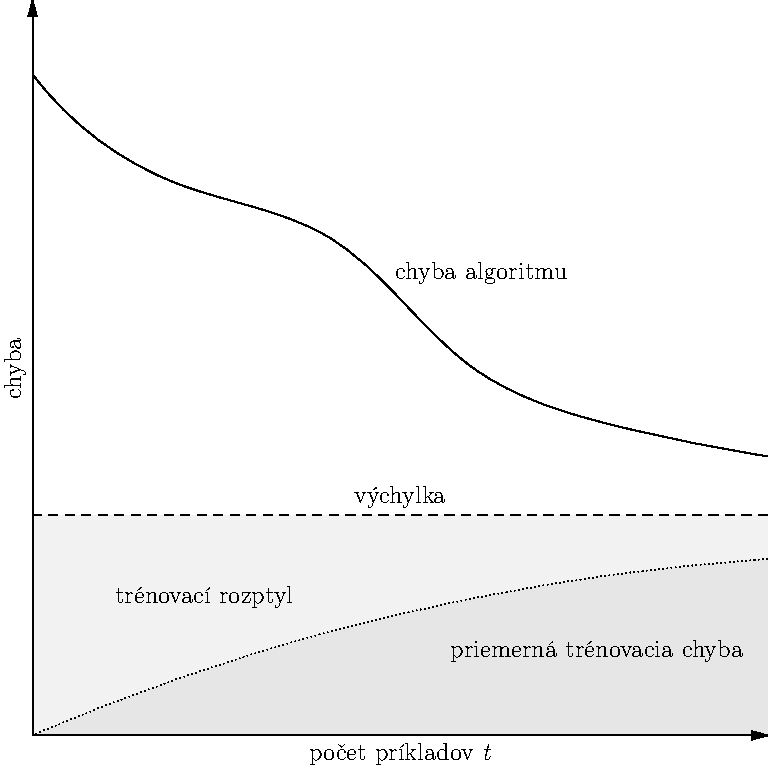
\includegraphics[scale=0.8]{obrazky/krivky1.pdf}
  \caption{Závislosť chyby algoritmu od počtu trénovacích príkladov $t$.}
  \label{img:train}
\end{figure}

\begin{figure}
  \centering
  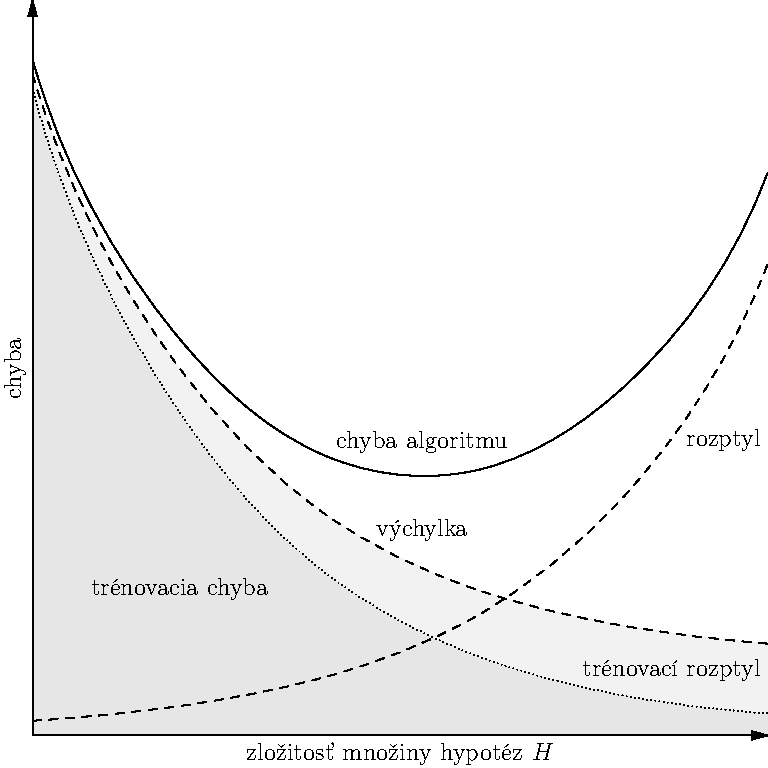
\includegraphics[scale=0.8]{obrazky/krivky2.pdf}
  \caption{Závislosť chyby algoritmu od zložitosti množiny hypotéz $H$.}
  \label{img:hypo}
\end{figure}

Obrázok \ref{img:train} vychádza z toho, že ak zvyšujeme počet
trénovacích príkladov, tak trénovací rozptyl aj rozptyl sa budú
znižovať (všimnite si, že výchylka závisí len od zložitosti množiny
hypotéz, ale nie od počtu trénovacích príkladov). Na základe vzťahu
(\ref{eq:vr2}) vieme teda povedať, že OTeCh sa bude so zvyšujúcim
počtom trénovacích príkladov približovať k výchylke zhora, kým OTrCh
sa bude postupne približovať k výchylke zdola. Preto pri fixnej
množine hypotéz nie je najzaujímavejším faktorom absolútna trénovacia
či testovacia chyba (ktorá obsahuje aj výchylku, ktorá je pri fixnej
množine hypotéz ireducibilná), ale rozdiel medzi trénovacou a
testovacou chybou.

Obrázok \ref{img:hypo} ilustruje situácie, ak máme fixné trénovacie
dáta $T$ a môžeme meniť zložitosť množiny hypotéz $H$.  Obrázok
demonštruje, že kľúčom ku dobre vyladenému modelu je nájdenie
rovnováhy medzi výchylkou a rozptylom (angl. \emph{bias-variance tradeoff}),
ktoré dohromady dávajú
testovaciu chybu.  Zložité $H$ bude mať malú výchylku ale veľký
rozptyl, čo vedie k tzv. \emph{preučeniu} (angl. \emph{overfitting}. V
takom prípade je potrebné zvýšiť množstvo trénovacích príkladov alebo
zjednodušiť množinu hypotéz. Jednoduché $H$ bude mať malý rozptyl, ale
veľkú výchylku a nastane tzv. \emph{podučenie}
(angl. \emph{underfitting}). V takom prípade nám zvýšenie počtu
trénovacích príkladov nepomôže, dominujúcim faktorom v testovacej
chybe je totiž malá reprezentačná sila množiny hypotéz $H$.

Na obrázku \ref{img:fitting} ilustrujeme oba koncepty. Úlohou je modelovať
kvadratickú funkciu, ku ktorej sme pridali malé množstvo šumu. Rozdelenie
$P$ teda vracia nejaké $x$ (napríklad z intervalu $\langle 0, 10 \rangle$)
a $y = x^2 + \varepsilon$, kde $\varepsilon$ je zvolené náhodne z intervalu
$\langle -1, 1 \rangle$. Ak za množinu hypotéz zvolíme lineárne funkcie,
vďaka ich jednoduchosti už pri malých trénovacích množinách bude trénovacia
chyba blízko očakávanej testovacej chyby (nízky rozptyl). Za to ale budú
všetky chyby vysoké (vysoká výchylka). Ak za množinu hypotéz zvolíme polynómy
nejakého vysokého stupňa, ľahko nájdeme polynóm presne prechádzajúci cez trénovacie
dáta (nízka trénovacia chyba), avšak mimo nich bude dávať výsledky úplne mimo
(vysoká testovacia chyba, a teda vysoký rozptyl).

\begin{figure}
  \centering
  \begin{subfigure}[b]{0.3\linewidth}
    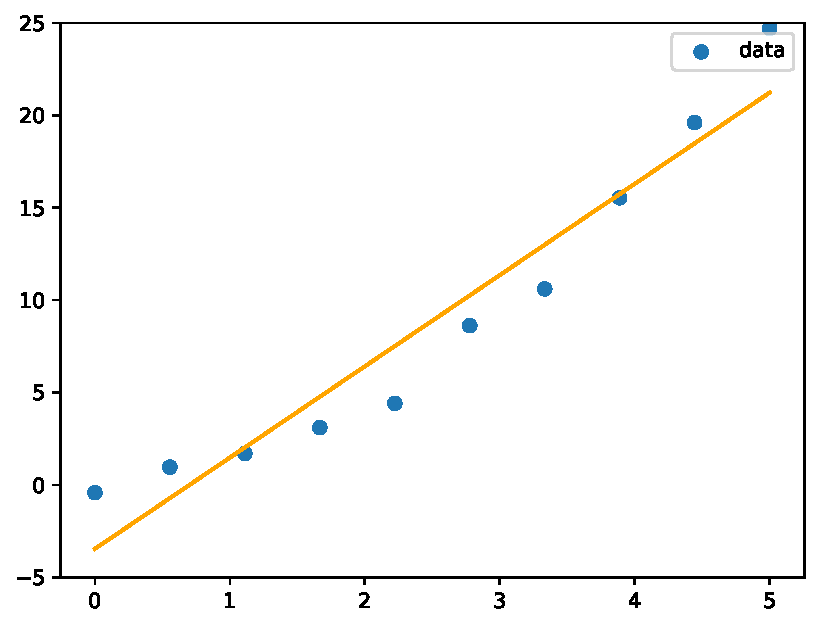
\includegraphics[width=\linewidth]{obrazky/fitting1.pdf}
  \end{subfigure}
  ~
  \begin{subfigure}[b]{0.3\textwidth}
    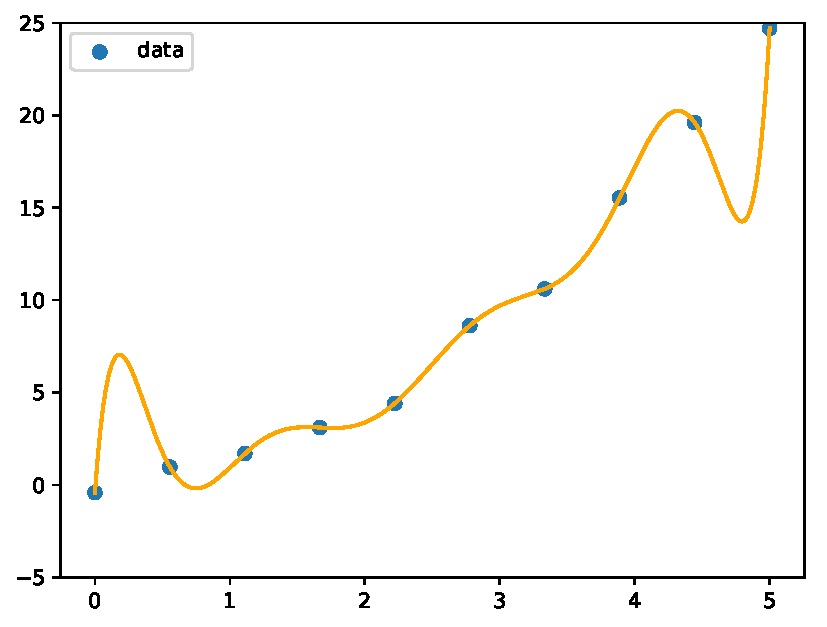
\includegraphics[width=\linewidth]{obrazky/fitting9.pdf}
  \end{subfigure}
  ~
  \begin{subfigure}[b]{0.3\textwidth}
    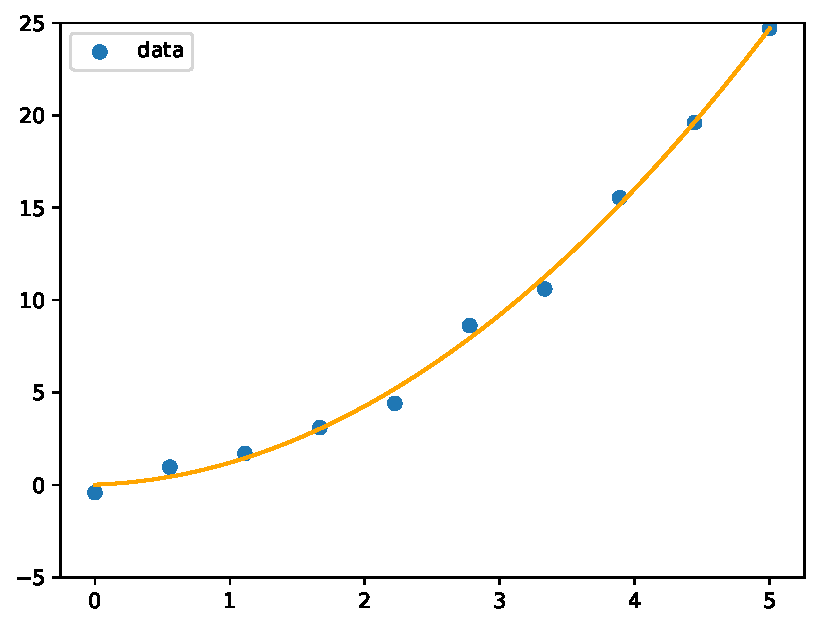
\includegraphics[width=\linewidth]{obrazky/fitting2.pdf}
  \end{subfigure}
  \caption{Podučenie, preučenie, akurát.}
  \label{img:fitting}
\end{figure}


\subsection{Regularizácia}

Predstavme si, že máme na výber z viacerých množín hypotéz $H_1, H_2, \ldots$,
čím ďalej tým zložitejších. Teda $H_1 \subseteq H_2 \subseteq H_3 \subseteq \ldots$.
Ak by sme si graficky znázornili testovacie a trénovacie chyby najlepších
hypotéz z jednotlivých množín, vyzeralo by to zhruba ako na obrázku
\ref{img:multimodels}.

\begin{figure}
  \centering
  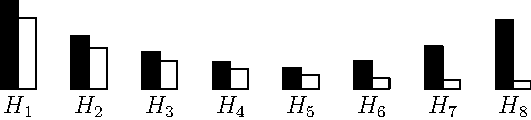
\includegraphics[scale=1]{obrazky/multimodels.pdf}
  \caption{Testovacie (čierne) a trénovacie (biele) chyby v čím ďalej,
    tým zložitejších množinách hypotéz $H$.}
  \label{img:multimodels}
\end{figure}

Z ktorej množiny hypotéz chceme vybrať? Pri trénovaní sa snažíme nájsť
hypotézu $h$, ktorá minimalizuje chybu na trénovacích dátach. Táto
chyba sa ale od očakávanej testovacej chyby líši zhruba
o $\rozptyl + \rozptylT$ (v očakávanom prípade).

V prístupe zvanom \emph{regularizácia} do minimalizovaného výrazu umelo
pridáme \emph{pokutu}, ktorá aproximuje $\rozptyl + \rozptylT$. Tento člen
označíme $\Lambda(h)$. Z čím zložitejšej množiny hypotéza $h$ je, tým
väčšia bude pokuta. Výstupom algoritmu potom je
$$\hat{h}_T = \argmin_{h \in H_1 \cup H_2 \cup \ldots} \left( \Err_T(h) + \Lambda(h) \right).$$

Uvedomme si, že vrámci jednej množiny $H_i$ ostáva ako najlepšia
hypotéza stále tá istá, ako pred zavedením pokuty. V jednej množine
sú totiž všetky hypotézy penalizované rovnako, nerobí to teda rozdiel.
Penalizácia nám ale umožňuje ``férovejšie'' porovnávať hypotézy z rôznych
množín, nakoľko bez pokuty by na tom boli (neprávom) lepšie
zložitejšie hypotézy.

Množiny $H_i$ nemusia byť explicitné, môžu byť implicitne skryté v tom,
aký tvar má výraz $\Lambda(h)$. Do jednej množiny patria tie hypotézy,
ktoré majú rovnakú penalizáciu.

Vo všetkých prípadoch je pokuta parametrizovaná reálnym
parametrom $\lambda$ hovoriacim, ako veľké pokuty chceme udeľovať.
Veľké $\lambda$ (v porovnaní s trénovacou chybou) nám hovorí, že sa
snažíme hlavne dosiahnuť jednoduché hypotézy; s malým $\lambda$ zas
kladieme dôraz na hypotézy s menšou trénovacou chybou.

Uvedieme si niekoľko príkladov výrazov, ktoré sú bežne používané ako
pokuta. Budeme predpokladať, že celá množina hypotéz, z ktorej vyberáme
(tj. $H_1 \cup H_2 \cup \ldots$) je množina lineárnych funkcii
$\R^n \to \R$. Hypotézy majú teda tvar
$$h(x) = a_1x_1 + a_2x_2 + \ldots + a_nx_n.$$
\begin{itemize}
  \item $L_2$ regularizácia (známa aj ako \emph{ridge regression}).
    $$ \Lambda(h) = \lambda \cdot \norm{(a_1, a_2, \ldots, a_n)}^2 = \lambda \cdot (a_1^2 + a_2^2 + \ldots + a_n^2) $$
    Táto pokuta ``tlačí'' váhy nepotrebných atribútov do nuly, pričom
    väčšie váhy tlačí viac. Takže čím dôležitejší atribút, tým väčšiu
    váhu si môže dovoliť mať.
  \item $L_1$ regularizácia (známa aj ako \emph{lasso}).
    $$ \Lambda(h) = \lambda \cdot (|a_1| + |a_2| + \ldots + |a_n|) $$
    Opäť ``tlačíme'' nepotrebné atribúty do nuly, pričom ale všetky
    váhy tlačíme rovnako. To nám vie vynulovať nepotrebné atribúty,
    čo nám vie znížiť výpočtové nároky: nemusíme pri výpočte uvažovať
    tie členy, ktoré majú nulový koeficient.
\end{itemize}

\subsection{Holdout testing}

V tomto prístupe si rozdelíme dostupné dáta na dve časti:
trénovaciu množinu a \emph{validačnú množinu}. Pomocou validačnej
množiny budeme odhadovať testovacie chyby pre jednotlivé množiny
hypotéz, na základe ktorých zistíme, ktorá množina hypotéz je
pre náš problém najvhodnejšia. Konkrétnejšie:
\begin{enumerate}
  \item Trénovaciu množinu použijeme na natrénovanie hypotéz
    z jednotlivých množín.
  \item \label{holdout:step2} Ako odhad testovacej chyby jednotlivých
    hypotéz použijeme ich chybu na validačnej množine. Podľa týchto
    odhadov zistíme, ktorá množina hypotéz je pre náš problém najvhodnejšia.
  \item Použijeme všetky dáta, ktoré máme k dispozícii (tj. z trénovacej
    aj validačnej množiny), na natrénovanie najlepšej možnej hypotézy.
    Berieme samozrejme do úvahy iba hypotézy z tej množiny hypotéz, ktorú
    sme identifikovali ako najvhodnejšiu. Výsledná hypotéza je výstupom
    algoritmu.
\end{enumerate}
 
V kroku \ref{holdout:step2} je dôležité, aby bola validačná
množina nezávislá od trénovacej. Prečo je to dôležité? Môžeme uvažovať
extrémny prípad, keď je validačná množina totožná s trénovacou. Potom
ale ako náš ``odhad'' dostaneme trénovaciu chybu, ktorá rozhodne nie
je dobrým odhadom testovacej chyby. Nezávislosť nám teda zaručuje, že
odhad získaný na validačnej množine je dobrý.

\emph{$k$-fold evaluation.} Pri holdout testovaní je dôležité mať
dobrý odhad testovacej chyby pre jednotlivé množiny hypotéz. Dát ale
môže byť málo, a v takom prípade môže byť odhad nestabilný/nepresný.
Môžeme ale experiment zopakovať niekoľkokrát: v každej iterácii teda
zvolíme inú trénovaciu a inú validačnú množinu, a dostaneme iný odhad
testovacej chyby. Keď tieto odhady spriemerujeme, dostaneme oveľa
presnejší odhad, ako keby sme vykonali iba jednu iteráciu.
V tomto konkrétnom prístupe je $k$ iterácii, a množiny sa volia
nasledovne: všetky dáta sa rozdelia na $k$ zhruba rovnako veľkých
a navzájom nezávislých množín $K_1, K_2, \ldots, K_k$. Následne,
v iterácii $i$ sa ako validačné dáta použije množina $K_i$. Všetko
ostatné budú trénovacie dáta.

\emph{Leave-one-out.} Ak chceme zmerať testovaciu chybu
výstupnej hypotézy, musíme si na to rezervovať ďalšiu časť dát:
\emph{testovaciu množinu}. Tú nepoužívame ani pri trénovaní, ani
pri validácii. Iba úplne na konci celého procesu na nej vypočítame
chybu výslednej hypotézy.




\subsection{Cvičenia}

V nasledujúcich dvoch cvičeniach môžete predpokladať, že trénovací
algoritmus vždy vráti nejakú funkciu (nemusí byť len jedna)
s minimálnou chybou na trénovacích dátach.

\begin{exercise}
  Je rozumné predpokladať, že s väčším množstvom trénovacích dát sa nám
  bude testovacia chyba zmenšovať. Sú ale zostrojiteľné situácie, kedy
  tomu tak nie je. Nájdite jednu takú situáciu.
  
  Konkrétne, nájdite takú množinu hypotéz $H$ funkcii $\R^n \to \R$
  a rozdelenie $P$, pre ktoré sa bude $\Err(\hat{h}_T)$ so zvyšujúcim
  sa počtom trénovacích chýb \emph{zvyšovať}. Na množinu hypotéz je
  kladená jedna podmienka: pre každú možnú trénovaciu množinu $T$
  musí existovať hypotéza v $H$, ktorá minimalizuje trénovaciu chybu.
  (Teda vždy musí existovať minimum, môže ich byť ale viac. Pre všeobecné
  $H$ vieme povedať iba to, že existuje infimum.)
\end{exercise}

\begin{exercise}
  Za určitých podmienok ale skutočne platí, že viac trénovacích dát
  nám vo veľkom merítku neuškodí. Nech množina hypotéz $H$ je konečná
  a všetky jej funkcie ($\R^n \to \R$) sú ohraničené. Dokážte, že
  pre $t \to \infty$ sa bude OTeCh hypotézy $\hat{h}_T$ blížiť k
  OTeCh najlepšej možnej hypotézy $h^\star$. Inak zapísané, dokážte
  $$\lim_{t \to \infty} \E_T \left[ \Err(\hat{h}_T) - \Err(h^\star) \right] = 0.$$
\end{exercise}

\begin{comment}
\begin{exercise}
  Dokážte korektnosť druhého technického kroku, v odvodení rozkladu
  výchylky na trénovací rozptyl a očakávanú trénovaciu chybu. Konkrétnejšie,
  dokážte
  $$ \E_T \left[ \E_{x_i, y_i} \left[ (h^\star(x_i) - \hat{h}(x_i)) \cdot (\hat{h}(x_i) - y_i) \right] \right] = 0. $$
  Predpoklady kladené na množinu hypotéz sú rovnaké: musí byť uzavretá
  na lineárne kombinácie a na limity.
\end{exercise}
\end{comment}

\begin{exercise}
  Jednou výhodou $L_2$ regularizácie oproti $L_1$ regularizácie je, že
  sa ľahšie minimalizuje výsledný výraz. Ako príklad uvedieme lineárnu
  regresiu. V nej je hypotéza parametrizovaná stĺpcovým vektorom
  $\theta = (\theta_1, \ldots, \theta_n)^T$. Výstupom pre vstup
  $x = (x_1, \ldots, x_n)$ je $x \cdot \theta$. 
  
  Označme $X$ maticu, ktorej riadkami sú vstupy jednotlivých trénovacích
  príkladov. Ďalej nech $y$ je stĺpcový vektor cieľových výstupov na
  jednotlivých príkladoch. Je známe, že optimálnymi parametrami
  lineárnej hypotézy je taký stĺpcový vektor $\theta$, ktorý je riešením
  rovnice
  $$X^T X \cdot \theta = X^T y.$$
  Dokáže, že keď k minimalizovanej hodnote pridáme pokutu vo forme
  $\lambda \cdot \norm{\theta}^2$, tak sa optimálnymi parametrami stane
  $\theta$ riešiaca rovnicu
  $$(X^T X + \lambda I) \cdot \theta = X^T y.$$
  Rozmyslite si tiež, že takéto explicitné vyjadrenie nie je možné
  priamočiaro získať pre $L_1$ regularizáciu.
\end{exercise}

\subsection{*** Rozklad na výchylku a rozptyl (ako štatistické pojmy)}
\label{biasvariance2}

V literatúre pod názvom \emph{bias-variance tradeoff} vystupuje odlišný
výsledok, ako vyššie spomenutý bias-complexity tradeoff. Uvádzame ho,
pretože sa často zamieňajú a je v tom zmätok. Pokúsime sa vyjasniť, kde
sú rozdiely medzi týmito dvomi výsledkami.

\begin{theorem}
  Zamerajme sa na jeden konkrétny vstup $x$, a merajme chybu výslednej
  hypotézy $\hat{h}_T$ iba na tomto vstupe. (Stále ale môžeme dostať
  rôzne $y$.) Na meranie chyby použijeme kvadratickú odchýlku. Označme
  očakávanú hodnotu tejto chyby (cez všetky možné trénovacie
  množiny $T$ a výstupy $y$) ako $\Err_{|x=x}(L)$. Tvrdíme, že
  sa dá vyjadriť nasledovne:
  $$
    \Err_{|x=x}(L)
      = \underbrace{\Var_T \left( \hat{h}_T(x) \right)}_{\text{\normalfont rozptyl}}
      + \underbrace{\left( \E_T \left[ \hat{h}_T(x) \right] - h^\square(x) \right)^2}_{\text{\normalfont výchylka}^2}
      + \underbrace{\E_y \left[ \varepsilon^2 \right]}_{\text{\normalfont šum}},
  $$
  kde $\varepsilon := y - h^\square(x)$.
\end{theorem}

Zastavme sa najprv nad tým, ako toto tvrdenie interpretovať. Pre každú
možnú vzorku trénovacích dát $T$ dostaneme nejakú inú hypotézu $\hat{h}_T$.
Rozptyl je nízky práve vtedy, keď budú všetky tieto hypotézy dávať
podobné výsledky. Ak je vysoký, znamená to, že výsledná hypotéza je
veľmi citlivá na trénovacie dáta; oplatí sa preto zväčšiť ich množstvo.
(Ak chceme byť veľmi skeptický, nič nezaručuje, že zväčšením trénovacej
množiny sa rozptyl zníži. Možno existuje iný dôvod, kvôli ktorému je
vysoký; takmer určite sa dajú skonštruovať takéto umelé protipríklady.)

Keď už uvažujeme všetky možné výsledné hypotézy $\hat{h}_T$, môžme sa
pozrieť na to, aký je ich ``priemerný odhad'': ak by sme spriemerovali
všetky ich výsledky, čo by sme dostali? Presne $\E_T [ \hat{h}_T(x) ]$;
výchylka-na-druhú potom meria, o koľko sa takáto priemerná hypotéza líši od
najlepšej možnej funkcie $h^\square$. Ak je výchylka vysoká ale variancia
nízka, znamená to, že takmer všetky $\hat{h}_T$ majú problém na vstupe $x$,
treba teda zvážiť voľbu zložitejšej množiny hypotéz.

Nakoniec, šum zodpovedá ireducibilnej chybe, ktorú bude mať každá hypotéza.
Je to v dôsledku toho, že jednému $x$ môže pripadať viacero rôznych $y$.
Presne túto chybu nadobúda najlepšia hypotéza-funkcia $h^\square$ (pre
ktorú sú rozptyl aj výchylka-na-druhú nulové).

\begin{proof}
  Upravujme pôvodný výraz.
  \begin{align}
    \Err_{|x=x}(L)
      &= \E_{T, y} \left[ (\hat{h}_T(x) - y)^2 \right] \\
      &= \E_{T, y} \left[ ((\hat{h}_T(x) - h^\square(x)) - \varepsilon)^2 \right] \\
      &= \E_{T, y} \left[ (\hat{h}_T(x) - h^\square(x))^2 + \varepsilon^2 - 2 \cdot \varepsilon \cdot (\hat{h}_T(x) - h^\square(x)) \right] \label{align:roznasob} \\
      &= \E_T \left[ (\hat{h}_T(x) - h^\square(x))^2 \right] + \E_y \left[ \varepsilon^2 \right] - \E_{T, y} \left[ 2 \cdot \varepsilon \cdot (\hat{h}_T(x) - h^\square(x)) \right] \label{align:linearita} \\
      &= \E_T \left[ (\hat{h}_T(x) - h^\square(x))^2 \right] + \E_y \left[ \varepsilon^2 \right] - 2 \cdot \E_y \left[ \varepsilon \right] \cdot \E_T \left[ (\hat{h}_T(x) - h^\square(x)) \right] \label{align:sucin_nezavislych} \\
      &= \E_T \left[ (\hat{h}_T(x) - h^\square(x))^2 \right] + \E_y \left[ \varepsilon^2 \right] \label{align:epsilon_nula}
  \end{align}
  Výraz sme upravili, potom v kroku \ref{align:roznasob} roznásobili a v kroku
  \ref{align:linearita} využili linearitu strednej hodnoty.
  Ďalej v kroku \ref{align:sucin_nezavislych} sme využili, že
  stredná hodnota súčinu nezávislých premenných je súčinom stredných
  hodnôt tých premenných. Nakoniec v kroku \ref{align:epsilon_nula}
  využívame $\E \left[ \varepsilon \right] = 0$. Zamerajme sa ďalej na prvý sčítanec.
  \begin{align}
    &= \E_T \left[ (\hat{h}_T(x) - h^\square(x))^2 \right] \\
    &= \E_T \left[ \hat{h}_T(x)^2 + h^\square(x)^2 - 2 \cdot \hat{h}_T(x) \cdot h^\square(x) \right] \label{align:roznasob2} \\
    &= \E_T \left[ \hat{h}_T(x)^2 \right] + \E_T \left[ h^\square(x)^2 \right] - \E_T \left[ 2 \cdot \hat{h}_T(x) \cdot h^\square(x) \right] \label{align:linearita2} \\
    &= \left( \Var_T \left( \hat{h}_T(x) \right) + \E_T \left[ \hat{h}_T(x) \right]^2 \right) + \left( \Var_T \left( h^\square(x) \right) + \E_T \left[ h^\square(x) \right]^2 \right) - \E_T \left[ 2 \cdot \hat{h}_T(x) \cdot h^\square(x) \right] \label{align:var_alt} \\
  \end{align}
  V kroku \ref{align:roznasob2} sme výraz roznásobili a potom v kroku
  \ref{align:linearita2} využili linearitu strednej hodnoty. V poslednom
  kroku (\ref{align:var_alt}) sme využili vzťah $\Var(a) = \E \left[ a^2 \right] - \E \left[ a \right]^2$.
  Pokračujme ďalej v úpravách.
  \begin{align}
    &= \left( \Var_T \left( \hat{h}_T(x) \right) + \E_T \left[ \hat{h}_T(x) \right]^2 \right) + h^\square(x)^2 - 2 \cdot \E_T \left[ \hat{h}_T(x)  \right] \cdot h^\square(x) \label{align:square_const} \\
    &= \Var_T \left( \hat{h}_T(x) \right) + \left( \E_T \left[ \hat{h}_T(x) \right]^2 + h^\square(x)^2 - 2 \cdot \E_T \left[ \hat{h}_T(x)  \right] \cdot h^\square(x) \right) \\
    &= \Var_T \left( \hat{h}_T(x) \right) + \left( \E_T \left[ \hat{h}_T(x) \right] - h^\square(x) \right)^2
  \end{align}
  V kroku \ref{align:square_const} sme využili, že $x$ je vopred dané,
  a teda $h^\square(x)$ je konštanta. Má teda nulový rozptyl a jeho
  stredná hodnota je identická s jeho hodnotou. Ďalej sme už len
  upravovali. Keď to celé dáme do jednej rovnice, dostaneme
  $$
    \Err_{|x=x}(L)
      = \underbrace{\Var_T \left( \hat{h}_T(x) \right)}_{\text{\normalfont rozptyl}}
      + \underbrace{\left( \E_T \left[ \hat{h}_T(x) \right] - h^\square(x) \right)^2}_{\text{\normalfont výchylka}^2}
      + \underbrace{\E_y \left[ \varepsilon^2 \right]}_{\text{\normalfont šum}}.
  $$
\end{proof}




